\chapter{Desarrollo}

A continuaci\'on se describe de forma detallada, el dise\~no y desarrollo del paquete MOMOS (Materia Organica y MicroOrganismos del Suelo), siguiendo la metodolog\'ia descrita en el cap\'itulo 3.

\section{Creación del esqueleto del paquete}

Para esta fase se utiliza el ambiente de desarrollo RStudio, el cual es un entorno de desarrollo integrado de fuente abierta para R que agrega muchas caracter\'isticas y herramientas de productividad, adem\'as de facilitar el uso de R, integrando la ayuda y la documentaci\'on.\\

En esta primera etapa se crea la estructura del paquete, además, se cargan los paquetes necesarios del CRAN de R (Repositorios de R), de los cuales depende MOMOS; los mismos fueron almacenados en el repositorio local que se crea para este paquete durante el proceso de desarrollo, y para el manejo de versiones se utiliza Git y GitHub, los principales paquete empleados son:\\

\begin{itemize}
    \item devtools(Wickham, H. \textit{et. al,} 2022; disponible en \url{https://cran.r-project.org/web/packages/devtools/index.html})
    \item roxygen2(Wickham, H. \textit{et. al,} 2022; disponible en \url{https://cran.r-project.org/web/packages/roxygen2/index.html})
    \item testthat(Wickham, H. \textit{et. al,} 2022; disponible en \url{https://cran.r-project.org/web/packages/testthat/index.html})
    \item RUnit(Burger, M. \textit{et. al,} 2018; disponible en \url{https://cran.rstudio.com/web/packages/RUnit/index.html})
    \item ggplot2(Wickham, H. \textit{et. al,} 2022; disponible en \url{https://cran.r-project.org/web/packages/ggplot2/index.html})
    \item reshape2(Wickham, H. \textit{et. al,} 2020; disponible en \url{https://cran.r-project.org/web/packages/reshape2/index.html})
    \item deSolve(Soetaert, K. \textit{et. al,} 2022; disponible en \url{https://cran.r-project.org/web/packages/deSolve/index.html})
    \item minpack.lm(Elzhov, T. \textit{et. al,} 2022; disponible en \url{https://cran.r-project.org/web/packages/minpack.lm/index.html})
    \item xlsx(Dragulescu A. \textit{et. al,} 2020; disponible en \url{https://cran.r-project.org/web/packages/xlsx/index.html})
    \item TODO: Agregar FME ( >= 1.3.6.2), knitr ( >= 1.40), rmarkdown ( >= 2.17)
\end{itemize}

\noindent
\textbf{Los pasos para la creación del esqueleto del paquete son los siguientes:\\}

\begin{itemize}
    \item Como se muestra en la Figura 4.1, dentro del entorno R Studio, en el men\'u principal, se selecciona la opci\'on \textit{''File''} y en el submen\'u desplegado se selecciona \textit{''New Project...''}
    \begin{figure}[H]
        \centering
          \begin{minipage}{0.8\textwidth}
            \centering
            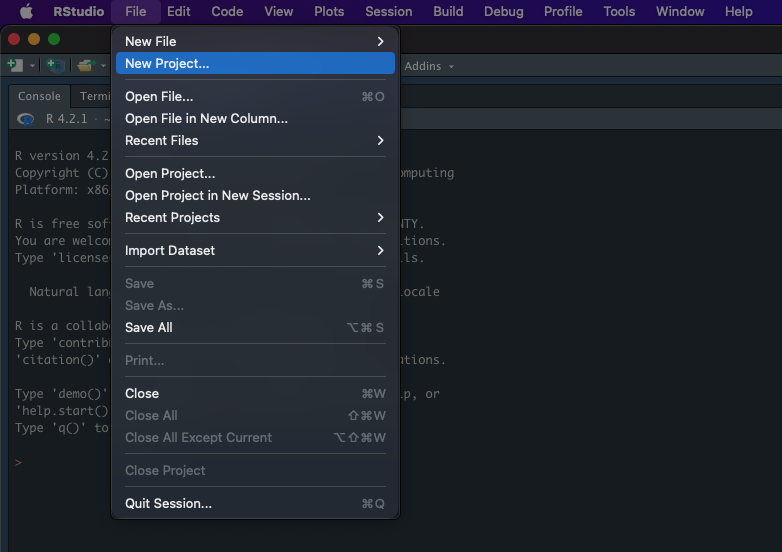
\includegraphics[width=0.8\textwidth]{figure_4_1.png}
            \caption{Nuevo proyecto}
            \label{fig:descripcion}
          \end{minipage}%
          \hspace{5mm}
    \end{figure}
    \item En la Figura 4.2, se selecciona la opci\'on \textit{''New Directory''}
    \begin{figure}[H]
        \centering
          \begin{minipage}{0.8\textwidth}
            \centering
            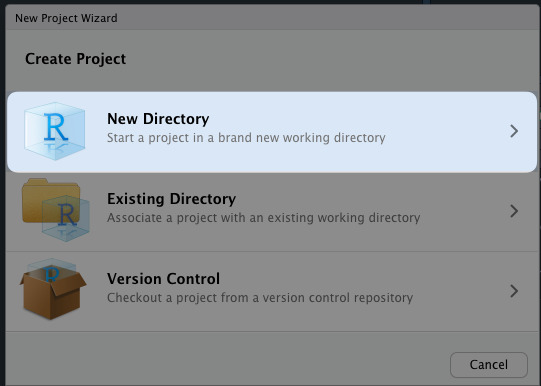
\includegraphics[width=0.8\textwidth]{figure_4_2.png}
            \caption{Nuevo directorio}
            \label{fig:descripcion}
          \end{minipage}%
          \hspace{5mm}
    \end{figure}
    \item En la figura 4.3, se selecciona la opci\'on \textit{''R Package''}
    \begin{figure}[H]
        \centering
          \begin{minipage}{0.8\textwidth}
            \centering
            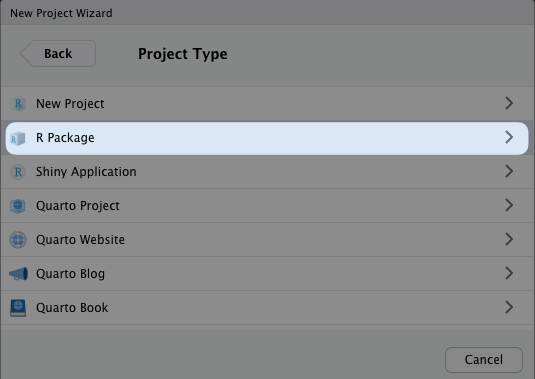
\includegraphics[width=0.8\textwidth]{figure_4_3.png}
            \caption{Tipo de proyecto}
            \label{fig:descripcion}
          \end{minipage}%
          \hspace{5mm}
    \end{figure}
    \item En la figura 4.4, se asigna el nombre del paquete y se selecciona el directorio donde es trabajado, posteriormente se presiona el bot\'on \textit{''Create Project''}
    \begin{figure}[H]
        \centering
          \begin{minipage}{0.8\textwidth}
            \centering
            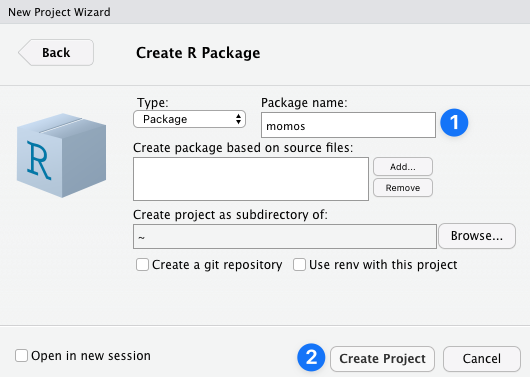
\includegraphics[width=0.8\textwidth]{figure_4_4.png}
            \caption{Nombre del paquete y directorio de trabajo}
            \label{fig:descripcion}
          \end{minipage}%
          \hspace{5mm}
    \end{figure}
    \item En la figura 4.5, se observa la descripci\'on del paquete
    \begin{figure}[H]
        \centering
          \begin{minipage}{0.8\textwidth}
            \centering
            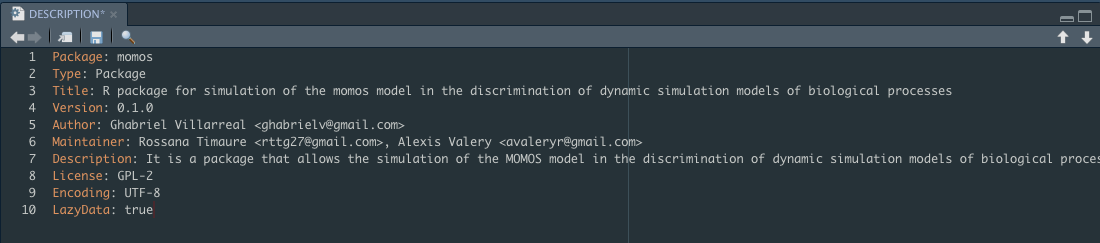
\includegraphics[width=1\textwidth]{figure_4_5.png}
            \caption{Estructura archivo DESCRIPTION}
            \label{fig:descripcion}
          \end{minipage}%
          \hspace{5mm}
    \end{figure}
    \item En la figura 4.6, finalmente se observa el esqueleto del paquete
    \begin{figure}[H]
        \centering
          \begin{minipage}{0.8\textwidth}
            \centering
            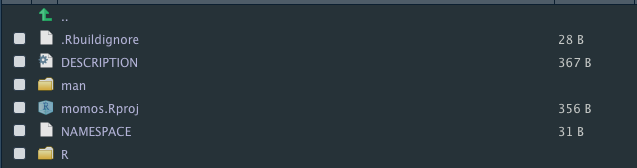
\includegraphics[width=1\textwidth]{figure_4_6.png}
            \caption{Esqueleto del paquete}
            \label{fig:descripcion}
          \end{minipage}%
          \hspace{5mm}
    \end{figure}
\end{itemize}

\noindent

\section{Registrar el m\'etodo para el env\'io y uso de funciones}

Se determina que la funci\'on principal reciba una lista de par\'ametros de entrada que sirven para calcular los valores de simulaci\'on del modelo, estos pueden ser opcionales, y todos deben ser num\'ericos, en caso de que no se defina alg\'un par\'ametro se cargan los valores por defecto correspondientes.\\

TODO: Agregar lista de parametros por defecto (tabla)

La primera función es \textit{calculate\textunderscore{momos()}} cuya salida muestra los valores de CM y RA simulados por cada instante de tiempo en un intervalo determinado, esta salida Figura 4.7 es un \textit{data frame} que corresponde a los datos simulados por el modelo din\'amico. Entendi\'endose como un data frame seg\'un Santana y Nieves (2014) “una clase de objetos especial en R. Normalmente, cuando se realiza un estudio estad \'istico sobre los sujetos u objetos de una muestra, la informaci\'on se organiza en un dataframe: una hoja de datos, en los que cada fila corresponde a un sujeto y cada columna a una variable. La estructura de un data frame es muy similar a la de una matriz. La diferencia es que una matriz s\'olo admite valores num\'ericos, mientras que en un data frame podemos incluir tambi\'en datos alfanum\'ericos."\\

Por lo tanto, para esta funci\'on desarrollada, las columnas del data frame corresponden a las variables de estudio (CM / RA) (TODO: Agregar definicion de CM / RA) y las filas a los valores de las mismas en cada intervalo de tiempo.\\

El modelo din\'amico genera una salida sin calibrar, esto puede producir que al comparar los datos reales con los datos simulados exista una gran diferencia entre los datos, por esta raz\'on, se decide diseñar una segunda función \textit{calibrate\textunderscore{momos()}} para realizar la calibración de los par\'ametros de entrada que afectan directamente las variables de salida (CM / RA), esto con el fin de buscar los valores ideales usando el algoritmo de levenberg marquart (TODO: Agregar informacion del algoritmo), con estos nuevos valores Figura 4.8 se busca asegurar un margen de error menor.\\

Adicionalmente, el resultado de esta funci\'on muestra tambi\'en los valores ideales de los par\'ametros que fueron usados para calibrar el modelo iterando nuevamente sobre la función \textit{calculate\textunderscore{momos()}}.\\

Para representar los valores obtenidos de las funciones anteriormente indicadas se define la funci\'on \textit{graph\textunderscore{momos()}} la cual tiene como finalidad comparar de manera grafica la curva del modelo con los valores simulados iniciales, los valores reales y tambi\'en los nuevos valores simulados despu\'es de la calibraci\'on.\\

Por \'ultimo, para unificar todas las funciones y mejorar el uso del paquete se crea la funci\'on \textit{momos()} que contempla todas las salidas de dichas funciones.

\begin{figure}[H]
    \centering
      \begin{minipage}{0.75\textwidth}
        \centering
        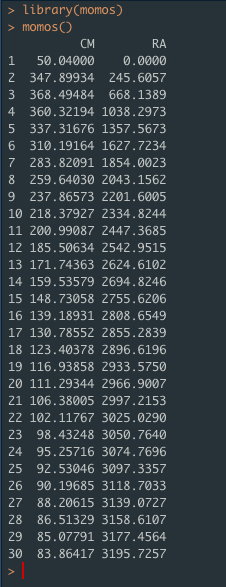
\includegraphics[width=0.5\textwidth]{figure_4_7.png}
        \caption{Datos de s\'alida sin calibrar}
        \label{fig:Fig}
      \end{minipage}%
      \hspace{5mm}
\end{figure}

\begin{figure}[H]
    \centering
      \begin{minipage}{0.75\textwidth}
        \centering
        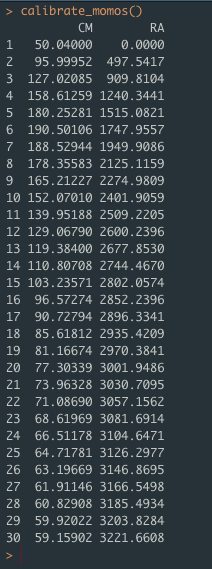
\includegraphics[width=0.5\textwidth]{figure_4_8.png}
        \caption{Datos de s\'alida calibrados}
        \label{fig:Fig}
      \end{minipage}%
      \hspace{5mm}
\end{figure}

\section{Dise\~no y codificaci\'on de las funciones}

La codificaci\'on de las funciones se realizaron en el IDE(Entorno de desarrollo integrado) RStudio, siguiendo las especificaciones algor\'itmicas detalladas en sus respectivos diagramas de flujo.

\noindent
\textbf{Diseño de las soluciones algor\'itmicas, para el c\'alculo del modelo momos}\\

El objetivo funcional de \textit{calculate\textunderscore{momos()}} es obtener los valores resultantes de la ejecuci\'on de MOMOS planteado por Valery (2018) para ello es necesario establecer los valores por defecto de los par\'ametros y constantes facilitados por el autor del modelo de esta investigaci\'on o los definidos por el usuario del paquete:

\begin{figure}[H]
  \centering
    \begin{minipage}{0.8\textwidth}
      \centering
      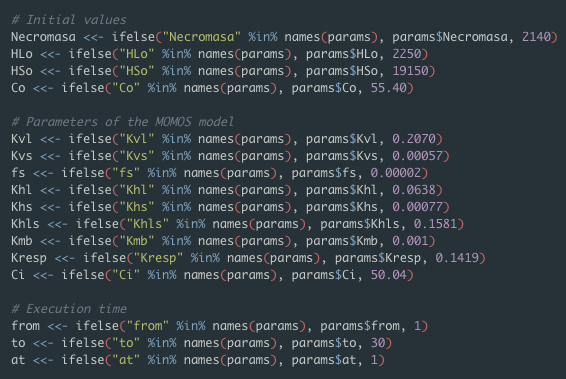
\includegraphics[width=0.8\textwidth]{figure_4_9.png}
      \caption{Establecer par\'ametros y constantes}
      \label{fig:Fig}
    \end{minipage}%
    \hspace{5mm}
\end{figure}

Los valores de los par\'ametros de tiempo de ejecuci\'on (from, to, at) indican la cantidad de veces y de datos que se debe iterar MOMOS. Adicionalmente, es necesario calcular los compartimientos de la necromasa labil (VL), necromasa estable (VS), carbono inicial de la biomasa microbiana (CM), humus labil (HL), humus estable (HS) y respiraci\'on inicial de la biomasa microbiana (RA) para obtener la funci\'on inicial.\\

\begin{figure}[H]
  \centering
    \begin{minipage}{0.6\textwidth}
      \centering
      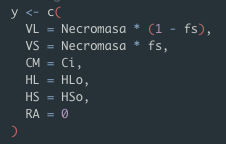
\includegraphics[width=0.6\textwidth]{figure_4_10.png}
      \caption{Establecer la funci\'on inicial y}
      \label{fig:Fig}
    \end{minipage}%
    \hspace{5mm}
\end{figure}

Posteriormente, se calculan las N derivadas de las funciones de los compartimientos anteriormente descritos, donde N es rango de cantidad de derivadas que se deben aplicar seg\'un los par\'ametros de tiempo de ejecuci\'on.\\

\begin{figure}[H]
  \centering
    \begin{minipage}{0.8\textwidth}
      \centering
      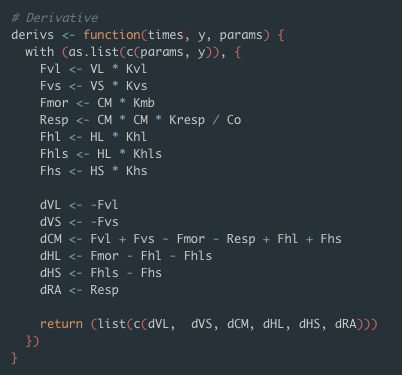
\includegraphics[width=0.8\textwidth]{figure_4_11.png}
      \caption{Funci\'on derivaci\'on}
      \label{fig:Fig}
    \end{minipage}%
    \hspace{5mm}
\end{figure}

Una vez se obtienen las N derivadas necesarias, se procede a utilizar la librer\'ia \textit{deSolve} haciendo uso de la funci\'on \textit{ode()} que resuelve un sistema de ecuaciones diferenciales ordinarias, dicha función recibe los siguientes par\'ametros: \\

\begin{itemize}
  \item \textit{func:} una función que calcula los valores de las derivadas en el sistema ODE (la definición del modelo) en el tiempo t.
  \item \textit{y:} estado inicial del sistema ODE.
  \item \textit{params:} par\'ametros que son recibidos por la funci\'on.
  \item \textit{times:} secuencia de tiempo para la salida deseada, el primer valor es el inicial.
  \item \textit{method:} m\'etodo de integraci\'on usado, en este caso usamos \textit{rk4} que el m\'etodo de \textit{Runge–Kutta}.
\end{itemize}

\begin{figure}[H]
  \centering
    \begin{minipage}{0.6\textwidth}
      \centering
      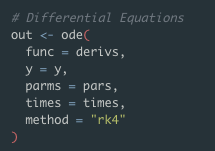
\includegraphics[width=0.6\textwidth]{figure_4_12.png}
      \caption{Ecuaci\'on diferencial}
      \label{fig:Fig}
    \end{minipage}%
    \hspace{5mm}
\end{figure}

Como resultado de la ecuaci\'on diferencial se obtienen los datos simulados por el modelo MOMOS en base a los par\'ametros y constantes establecidos, los cuales ser\'an \'utiles para calibrar y luego comparar en las funciones posteriores, entre los datos simulados, datos calibrados y datos experimentales.\\

\begin{figure}[H]
  \centering
    \begin{minipage}{0.55\textwidth}
      \centering
      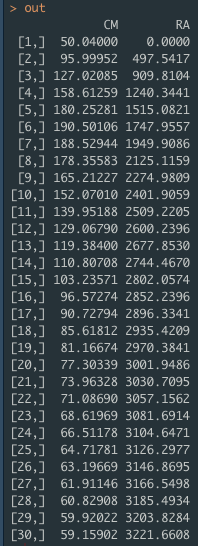
\includegraphics[width=0.55\textwidth]{figure_4_13.png}
      \caption{Resultado de la ecuaci\'on diferencial}
      \label{fig:Fig}
    \end{minipage}%
    \hspace{5mm}
\end{figure}

\noindent
\textbf{Diseño de las soluciones algor\'itmicas, para la calibraci\'on del modelo momos}\\

El objetivo funcional de \textit{calibrate\textunderscore{momos()}} es obtener al menos un par\'ametro que pueda ser calibrado para encontrar su valor ideal, el cual permita que los datos simulados se acerquen a los datos experimentales, logrando asi un margen de error que sea tolerante para la investigaci\'on.\\

En este caso se implementa el algoritmo de \textit{levenberg-marquart} usando la librer\'ia de R \textit{minpack.lm} para resolver problemas de m\'inimos cuadrados no lineales donde este algoritmo parte de los datos experimentales, por esta raz\'on procedemos a leer los datos dentro de la funci\'on de calibraci\'on.\\

\begin{figure}[H]
  \centering
    \begin{minipage}{1\textwidth}
      \centering
      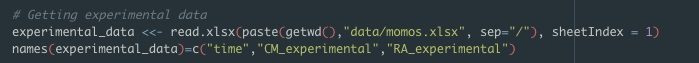
\includegraphics[width=1\textwidth]{figure_4_14.png}
      \caption{Extracci\'on de datos experimentales}
      \label{fig:Fig}
    \end{minipage}%
    \hspace{5mm}
\end{figure}

Para usar el algoritmo mencionado se debe crear un vector de residuos cuya suma cuadrada debe ser
minimizada, y el primer argumento debe ser par, asi que procedemos a crear una funci\'on que retorna ese vector, inicialmente, se debe hacer una uni\'on de los tiempos de ejecuci\'on entre los datos experimentales y simulados, donde el tiempo debe ser \'unico. Por otra parte, se establecen los par'ametros de estimaci\'on y se procede a calcular MOMOS para el valor indicado, luego se evaluan los valores estimados versus los valores experimentales para los tiempos donde ambos coinciden aplicando una intersecci'on entre los datos, finalmente, se restan los valores estimados con los valores experimentales, y se devuelve el vector a la funci\'on de calibraci\'on.\\

\begin{figure}[H]
  \centering
    \begin{minipage}{0.9\textwidth}
      \centering
      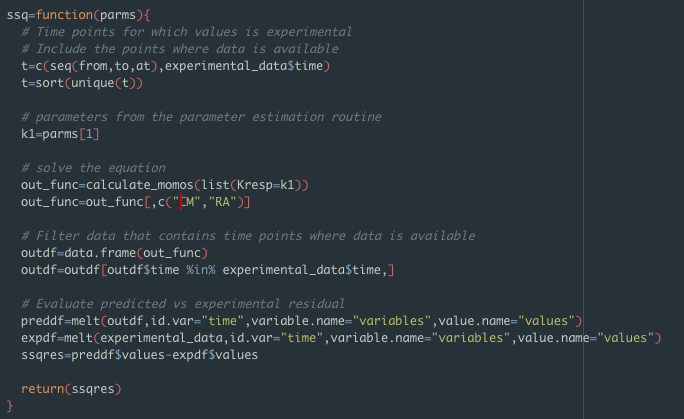
\includegraphics[width=0.9\textwidth]{figure_4_15.png}
      \caption{Creaci\'on del vector de residuos}
      \label{fig:Fig}
    \end{minipage}%
    \hspace{5mm}
\end{figure}

Seguidamente, se establece el par\'ametro que se desea calibrar, en este caso usamos \textit{Kresp}, despues de que el vector de residuos es creado se procede a llamar la función de ajuste, la cual devuelve la información con el valor ideal para el par\'ametro indicado.

\begin{figure}[H]
  \centering
    \begin{minipage}{0.8\textwidth}
      \centering
      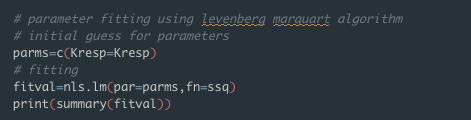
\includegraphics[width=0.8\textwidth]{figure_4_16.png}
      \caption{Encontrar el valor ideal del par\'ametro Kresp}
      \label{fig:Fig}
    \end{minipage}%
    \hspace{5mm}
\end{figure}

\begin{figure}[H]
  \centering
    \begin{minipage}{0.8\textwidth}
      \centering
      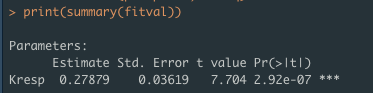
\includegraphics[width=0.8\textwidth]{figure_4_17.png}
      \caption{Valor ideal del par\'ametro Kresp}
      \label{fig:Fig}
    \end{minipage}%
    \hspace{5mm}
\end{figure}

Finalmente, el valor ideal es enviado como un nuevo par\'ametro a la funci\'on \textit{calculate\textunderscore{momos()}} para retorar como un dataframe los nuevos valores de MOMOS calibrados y cercanos a los valores experimentales.

\begin{figure}[H]
  \centering
    \begin{minipage}{0.5\textwidth}
      \centering
      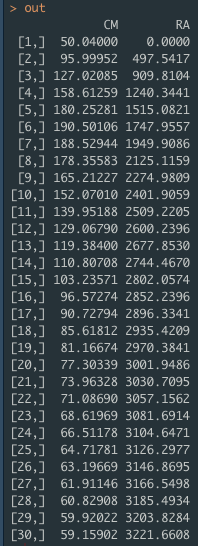
\includegraphics[width=0.5\textwidth]{figure_4_13.png}
      \caption{Dataframe con los datos calibrados de MOMOS}
      \label{fig:Fig}
    \end{minipage}%
    \hspace{5mm}
\end{figure}

\noindent
\textbf{Diseño de las soluciones algor\'itmicas, para la graficaci\'on del modelo momos}\\

El objetivo funcional de \textit{graph\textunderscore{momos()}} usando la librer\'ia de R \textit{ggplot2} es obtener una representaci\'on gr\'afica de los datos obtenidos durante el desarrollo de la investigaci\'on.\\

TODO: Agregar codigo de graficacion.

En ella se reflejan las curvas del modelo MOMOS para los diferentes tipos de datos: experimentales, simulados, calibrados.\\

TODO: Agregar grafica de las curvas del modelo MOMOS
\section{Pruebas unitarias de las funciones}

Lorem Ipsum is simply dummy text of the printing and typesetting industry. Lorem Ipsum has been the industry's standard dummy text ever since the 1500s, when an unknown printer took a galley of type and scrambled it to make a type specimen book. It has survived not only five centuries, but also the leap into electronic typesetting, remaining essentially unchanged. It was popularised in the 1960s with the release of Letraset sheets containing Lorem Ipsum passages, and more recently with desktop publishing software like Aldus PageMaker including versions of Lorem Ipsum.

\section{Chequear la carga del paquete}

Lorem Ipsum is simply dummy text of the printing and typesetting industry. Lorem Ipsum has been the industry's standard dummy text ever since the 1500s, when an unknown printer took a galley of type and scrambled it to make a type specimen book. It has survived not only five centuries, but also the leap into electronic typesetting, remaining essentially unchanged. It was popularised in the 1960s with the release of Letraset sheets containing Lorem Ipsum passages, and more recently with desktop publishing software like Aldus PageMaker including versions of Lorem Ipsum.

\section{Construcci\'on del m\'etodo de distribuci\'on del paquete}

Lorem Ipsum is simply dummy text of the printing and typesetting industry. Lorem Ipsum has been the industry's standard dummy text ever since the 1500s, when an unknown printer took a galley of type and scrambled it to make a type specimen book. It has survived not only five centuries, but also the leap into electronic typesetting, remaining essentially unchanged. It was popularised in the 1960s with the release of Letraset sheets containing Lorem Ipsum passages, and more recently with desktop publishing software like Aldus PageMaker including versions of Lorem Ipsum.
